\section{System Design}
We build a mobile bimanual robot equipped with two dexterous hands. To enable large-scale training in simulation, we also construct corresponding high-fidelity simulation models that accurately replicate the physical characteristics and kinematic structures of the real-world system.

\begin{figure}[t]
  \centering
  \vspace{-20pt}
  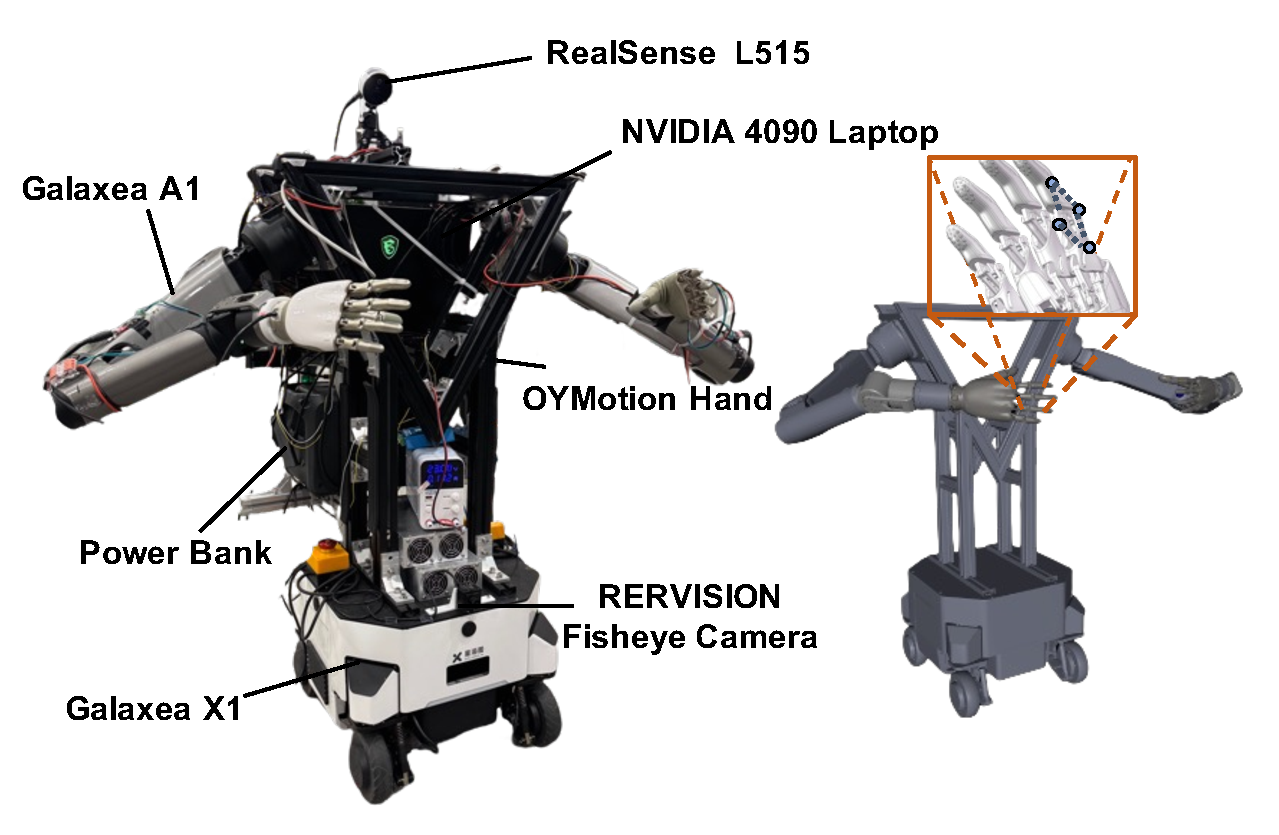
\includegraphics[width=1.0\linewidth]{figures/hardware.pdf}
  \vspace{-15pt}
  \caption{\textbf{System Design.} We construct a unified setup of mobile bimanual robots equipped with dexterous hands in both simulation and the real world. Through high-fidelity simulation, this robotic platform is capable of enabling sim2real transfer across a wide range of complex manipulation tasks.}
  \label{fig:system}
\end{figure}


\subsection{Hardware Design}
As shown in Figure~\ref{fig:system}, our robotic system is constructed by integrating an X1 mobile base, two 6-DoF Galaxea A1 arms, and two OYMotion 6-DoF dexterous hands. The torso part is assembled using lightweight aluminum alloy tubing to ensure structural rigidity. Additionally, we use a laptop with an NVIDIA RTX 4090 GPU for supporting ROS control and network inference. Regarding the camera, we adopt the RealSense L515 to capture RGBD observations and the RERVISION Fisheye camera for navigation. 

\subsection{Simulation Design}
We employ both the MuJoCo~\cite{todorov2012mujoco} and MJX simulation platforms~\cite{MJX} to construct training environments tailored for our mobile bimanual robotic system. The kinematic structure of the robot is carefully modeled, and relevant dynamic parameters are configured to ensure stable behavior in the simulation. The actuation range of each joint is configured to match that of the physical robot. For the dexterous hands, whose fingers contain passive joints not directly actuated by motors, we leverage MuJoCo’s capabilities for modeling closed chain mechanisms to faithfully simulate these passive DoFs, which achieves a high-fidelity reproduction of the hand's physical interactions. In contrast to the conventional approaches of simulating inter-link motion relationships through mimic joints or tendon-based mechanisms,  we utilize the equality constraint feature in MuJoCo to directly construct linkage structures as defined in the original CAD models. This formulation affords a more precise representation of the motion dependencies among passive DoFs, leading to a more faithful simulation of constrained multi-link dynamics.

Furthermore, to enhance the stability of interactions between the robot and manipulated objects, we restructure the collision modeling scheme. Rather than performing collision detection based directly on the original mesh representations of the objects and the hand, we approximate their geometries using primitive shapes. This abstraction facilitates more granular and stable collision computation. The Inverse Kinematics~(IK) control of the robotic system is implemented using the Mink library~\cite{ZakkaMink2025}. 






